\documentclass[12pt]{article}

\usepackage[T1]{fontenc} % Adjust font encoding to include symbols
\usepackage[dvipsnames]{xcolor} % Colors
\usepackage{amsmath} % Math
\usepackage{witharrows} % Equation Arrows
\usepackage[normalem]{ulem} % Strike-through Text
\usepackage{graphicx} % Images
\usepackage{titlesec} % Title Configuration
\usepackage{enumitem} % More Configurable enumerate
\usepackage{pifont} % More symbols

\usetikzlibrary{shapes.geometric} % Hexagons

\graphicspath{ {./images/} }

% Command to strike-through text in math equations
\newcommand{\cross}[1]{\text{\sout{\ensuremath{#1}}}}
% Adjust the format of subsection (#. )
\renewcommand{\thesubsection}{\arabic{subsection}.\hspace{0.2em}}
% Change subsub sections numbering to alphabetical (a))
\renewcommand{\thesubsubsection}{\thesubsection\alph{subsubsection})}
% Configure sub and subsub sections to display inline
\setcounter{secnumdepth}{3}
\titleformat{\subsection}[runin]
  {\normalfont\normalsize\bfseries}{\thesubsection}{0em}{}
\titleformat{\subsubsection}[runin]
  {\normalfont\normalsize\bfseries}{\thesubsubsection}{0.5em}{}
% Create new commands to reference exercises
\newcommand{\exercise}{\subsection{}\setcounter{subsubsection}{0}}
\newcommand{\multipartexercise}{\addtocounter{subsection}{1}\setcounter{subsubsection}{0}}
\newcommand{\exercisepart}{\subsubsection{}}

\title{
    COMP4097 Mobile Computing \linebreak
    Assignment 2
}
\author{Jonatan Juhas (19502966)}
\date{\today}

\begin{document}
\maketitle

\multipartexercise
\exercisepart
As the hamming code (7 4) requires a message length of 4, we split it into 2 parts: 1000 and 1010.

\bigskip
\noindent
The first part (assuming the pattern M7 M6 M5 P4 M3 P2 P1) is:

\begin{description}[labelwidth=0pt]
\item[]
\begin{DispWithArrows*}[format=cccccccr,fleqn,mathindent=0pt]
    1 &\ 0 &\ 0 &\ \_ &\ 0 &\ \_ &\ \_ &
    \Arrow{P1: $\_001 \rightarrow 0+0+1=1 \ (odd) \rightarrow 1001$} \\
    1 &\ 0 &\ 0 &\ \_ &\ 0 &\ \_ &\ 1 &
    \Arrow{P2: $\_001 \rightarrow 0+0+1=1 \ (odd) \rightarrow 1001$} \\
    1 &\ 0 &\ 0 &\ \_ &\ 0 &\ 1 &\ 1 &
    \Arrow{P4: $\_101 \rightarrow 1+0+1=2 \ (even) \rightarrow 0101$} \\
    1 &\ 0 &\ 0 &\ 0 &\ 0 &\ 1 &\ 1 &
\end{DispWithArrows*}
\end{description}

\noindent
The second part is:

\begin{description}[labelwidth=0pt]
\item[]
\begin{DispWithArrows*}[format=cccccccr,fleqn,mathindent=0pt]
    1 &\ 0 &\ 1 &\ \_ &\ 0 &\ \_ &\ \_ &
    \Arrow{P1: $\_001 \rightarrow 0+1+1=2 \ (even) \rightarrow 0011$} \\
    1 &\ 0 &\ 1 &\ \_ &\ 0 &\ \_ &\ 0 &
    \Arrow{P2: $\_001 \rightarrow 0+0+1=1 \ (odd) \rightarrow 1001$} \\
    1 &\ 0 &\ 1 &\ \_ &\ 0 &\ 1 &\ 0 &
    \Arrow{P4: $\_101 \rightarrow 1+0+1=2 \ (even) \rightarrow 0101$} \\
    1 &\ 0 &\ 1 &\ 0 &\ 0 &\ 1 &\ 0 &
\end{DispWithArrows*}
\end{description}

\noindent
So the message transmitted to Station B will be 1001011 1010010

\exercisepart
We receive 2 messages: 1011011 and 1011010.

\bigskip
\noindent
For the first message we check all parity bits:

\noindent
P1: $1011 \rightarrow 1+0+1+1=3 \ \color{Red} \ \text{\ding{55}}$ \\
P2: $1001 \rightarrow 1+0+0+1=2 \ \color{Green} \ \text{\ding{51}}$ \\
P4: $1101 \rightarrow 1+1+0+1=3 \ \color{Red} \ \text{\ding{55}}$

\noindent
Correcting the message with $\text{P1} + \text{P4} = 5$ to 1001011.

\bigskip
\noindent
We check the parity bits in the second message:

\noindent
P1: $0011 \rightarrow 0+0+1+1=2 \ \color{Green} \ \text{\ding{51}}$ \\
P2: $1001 \rightarrow 1+0+0+1=2 \ \color{Green} \ \text{\ding{51}}$ \\
P4: $1101 \rightarrow 1+1+0+1=3 \ \color{Red} \ \text{\ding{55}}$

\noindent
Correcting the message with $\text{P4} = 4$ to 1010010.

\exercisepart
We again receive 2 messages after the spike: 1100111 and 1011010.

\bigskip
\noindent
The first message check results in:

\noindent
P1: $1101 \rightarrow 1+1+0+1=3 \ \color{Red} \ \text{\ding{55}}$ \\
P2: $1111 \rightarrow 1+1+1+1=4 \ \color{Green} \ \text{\ding{51}}$ \\
P4: $0011 \rightarrow 0+0+1+1=2 \ \color{Green} \ \text{\ding{51}}$

\noindent
Correcting the message with $\text{P1} = 1$ to 1100110.

\bigskip
\noindent
The second message check:
\\
P1: $0011 \rightarrow 0+0+1+1=2 \ \color{Green} \ \text{\ding{51}}$ \\
P2: $1001 \rightarrow 1+0+0+1=2 \ \color{Green} \ \text{\ding{51}}$ \\
P4: $1101 \rightarrow 1+1+0+1=3 \ \color{Red} \ \text{\ding{55}}$

\noindent
Correcting the message with $\text{P4} = 4$ to 1010010.

\bigskip

The channel seems to be quite unreliable but we manage to fix all errors thanks to the hamming code encoding.

\multipartexercise
\exercisepart
The equation for calculating the rate can be summarized as:
\begin{align*}
  \frac{\text{payload bytes}*8*1000}{\text{\#slots}*0.625*1000}
\end{align*}

An ACL Link (Asynchronous Connection-Less) using DM5 and maximum number of bytes can achieve a rate of $\frac{224*8*1000}{5*0.625*1000} \approx 477.8kb/s$ as indicated in the table under asymmetric rate.

The reverse connection rate uses DM1 so we adjust the number of payload bytes to 17 and and number of slots to 1 so we get $\frac{17*8*1000}{1*0.625*1000} \approx 108.8kb/s$.

\exercisepart
$2Mb=2000kb$ so with a transfer speed of $477.8kbps$ we can transfer the image in $\approx4.1s$.

\exercisepart
Since the high quality stream requires a minimum transfer speed of $256kbps$, which is below our theoretical maximum of $477.8kbps$, the connection will be stable.

The "professional" grade mp3 transfer requires $512kbps$ transfer rate, which exceeds our limits. Certain packets will therefore come delayed or not at all which will result in stuttering in the audio.

\exercisepart
An SCO HV3 link only supports a maximum connection speed of $64kbps$, which is way below our limit. Most packets will not arrive at the slave on time or at all and will be dropped. The listening experience will be drastically diminished.

\multipartexercise
\exercisepart
Given the frequency reuse of 7 and a semi-random distribution of the initial cell frequencies (2-4-6-3-5-7) we construct a hexagonal latice as shown in figure \ref{celllayout}.

\begin{figure}[!h]
\centering
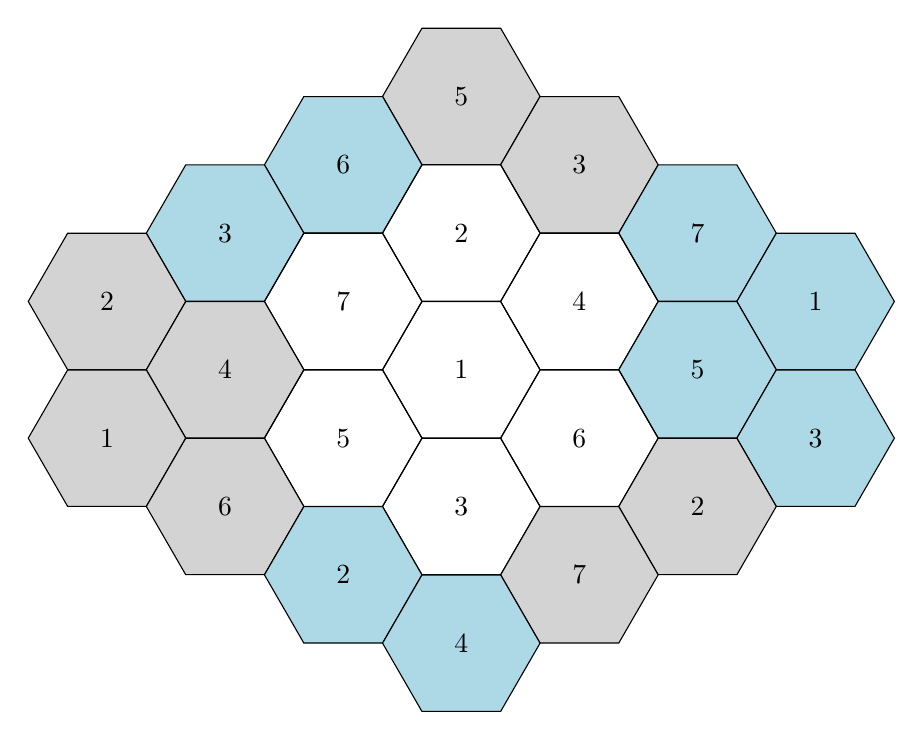
\begin{tikzpicture}[x=15mm,y=8.68mm]
  % Define colors for tikz
  \definecolor{lightblue}{RGB}{173, 216, 230}
  \definecolor{lightgray}{RGB}{211, 211, 211}
  % Configure hexagons
  \tikzset{
    box/.style={
      regular polygon,
      regular polygon sides=6,
      minimum size=20mm,
      inner sep=0mm,
      outer sep=0mm,
      rotate=0,
    draw
    }
  }

\node[box,fill=lightgray] at (2*2+1,2*2+1) {5};

\node[box,fill=lightblue] at (2*2,2*2) {6};
\node[box,fill=lightgray] at (2*3,2*2) {3};

\node[box,fill=lightblue] at (2*1+1,2*1+1) {3};
\node[box] at (2*2+1,2*1+1) {2};
\node[box,fill=lightblue] at (2*3+1,2*1+1) {7};

\node[box,fill=lightgray] at (2*1,2*1) {2};
\node[box] at (2*2,2*1) {7};
\node[box] at (2*3,2*1) {4};
\node[box,fill=lightblue] at (2*4,2*1) {1};

\node[box,fill=lightgray] at (2*1+1,2*0+1) {4};
\node[box] at (2*2+1,2*0+1) {1};
\node[box,fill=lightblue] at (2*3+1,2*0+1) {5};

\node[box,fill=lightgray] at (2*1,2*0) {1};
\node[box] at (2*2,2*0) {5};
\node[box] at (2*3,2*0) {6};
\node[box,fill=lightblue] at (2*4,2*0) {3};

\node[box,fill=lightgray] at (2*1+1,2*-1+1) {6};
\node[box] at (2*2+1,2*-1+1) {3};
\node[box,fill=lightgray] at (2*3+1,2*-1+1) {2};

\node[box,fill=lightblue] at (2*2,2*-1) {2};
\node[box,fill=lightgray] at (2*3,2*-1) {7};

\node[box,fill=lightblue] at (2*2+1,2*-2+1) {4};

\end{tikzpicture}
\caption{Suggested cell layout using frequency reuse of 7}
\label{celllayout}
\end{figure}

The cell area can be calculated as $1.5\sqrt{3}R^2$. Since our radius is 1km for each cell, one cell covers the surface of $\approx2.6km^2$. Our are consists of 23 segments which totals an area of $\approx59.8km^2$.

\exercisepart
In the past, before the cell architecture was introduced, a single antenna could only handle a specific amount of simultaneous connections - 25 channels on a high powered transmitter within an 80km reach.

By decreasing this reach and using more transmitters, that do not interfere with each other (such as 5G antennas), the effective amount of devices capable of connecting (let's say within a city) increases.
This is very important especially for the future of IoT technology.

\exercise
During paging the MTSO (Mobile Telecommunications Switching Office) tries to connect to a specific device and deliver a call. It sends a paging request to specific BS's within an area based on the number called, each transmitting it on their own channel.

The station to which the phone being called is connected then establishes connection.

\multipartexercise
\exercisepart
Given the chipping codes:\\
\begin{tabular}{lrrrr}
A:&-1&-1&-1&-1\\
B:&-1&-1&1&1\\
C:&-1&1&-1&1\\
\end{tabular}

Building a dot product we get $(-1*-1*-1)+(-1*-1*1)+(-1*1*-1)+(-1*1*1)=0$. Thus the 3 chipping codes are orthogonal and can be used for CDMA.

\exercisepart
For the first bit we generate the code for A (1), B (1) and C (0) by combining A and B's chipping codes and the inverse of C's chipping code (1 -1 1 -1):

\bigskip
\noindent
(-1-1+1) (-1-1-1) (-1+1+1) (-1+1-1) = -1 -3 1 -1

\bigskip
\noindent
The second bit pattern A (0) - inverse, B (1), C (1)\\
(1-1-1) (1-1+1) (1+1-1) (1+1+1) = -1 1 1 3

\bigskip
\noindent
The third bit pattern A (1), B (1), C (1)\\
(-1-1-1) (-1-1+1) (-1+1-1) (-1+1+1) = -3 -1 -1 1

\bigskip
\noindent
The receiver will receive the signal pattern D -1 -3 1 -1 | -1 1 1 3 | -3 -1 -1 1

\exercisepart
We take the input received and multiply it by A's chipping code:\\
$(-1*-1) + (-3*-1) + (1*-1) + (-1*-1) = 4$ so A must have sent a 1\\
$(-1*-1) + (1*-1) + (1*-1) + (3*-1) = -4$ so the second bit is 0\\
$(-3*-1) + (-1*-1) + (-1*-1) + (1*-1) = 4$ so the last bit was 1

\bigskip
\noindent
The bit pattern sent by A was therefore 101 which is indeed correct.

\exercisepart
We proceed as in the last part:\\
$(-1*-1) + (-3*-1) + (1*1) + (-1*1) = 4 \rightarrow 1$\\
$(-1*-1) + (1*-1) + (1*1) + (3*1) = 4 \rightarrow 1$\\
$(-3*-1) + (-1*-1) + (-1*1) + (1*1) = 4 \rightarrow 1$

\bigskip
\noindent
So the bit patter sent by B was 111

\multipartexercise
\exercisepart
We can convert the DMS (degrees, minutes, seconds) format into the decimal format by using the simple formula $d + \frac{m}{60} + \frac{s}{3600}$. The result will be $22 + \frac{15}{60} + \frac{16.9}{3600} = 22.25469\overline{4}$, $113 + \frac{54}{60} + \frac{15}{3600} = 113.9041\overline{6}$

\bigskip
\noindent
22.254694, 113.90417 (aka Tian Tan Buddha)

\exercisepart
The device can send a timestamp to the satellite and then wait for a response. The satellite sends the timestamp back and the device can then measure how long it took for the signal to travel to the satellite and back estimating the distance to it. If at least 3 satellites can be reached the location of the device can be triangulated by "drawing" a circle around each satellite with the radius of the calculated distance and finding the spot where they overlap.

Using more satellites leads to better positioning results as well as above sea height measurements.

\end{document}
